\documentclass[aspectratio=169,10pt]{beamer}\usetheme{default}\usecolortheme{seahorse}\setbeamertemplate{navigation symbols}{}\setbeamertemplate{footline}[frame number]
\usepackage[T1]{fontenc}\usepackage[utf8]{inputenc}\usepackage{helvet}\usepackage{booktabs,amsmath}
\setbeamertemplate{footline}{\hfill{\tiny\textcolor{red!70!black}{DRAFT for the author\textquoteright{}s review, November 12, 2026}\quad\insertframenumber}\hspace{1em}\vspace{0.4em}}
\title{Automobiles and curb along rue de Terrebonne}\subtitle{Registered vehicles known by postal district, modelled below it; legal curb measured block face by block face}\author{Rick Hoge, PhD}\institute{Terrebonne-open-sources}\date{November 12, 2026}
\begin{document}
\begin{frame}\titlepage\end{frame}
\begin{frame}{Overview}
\begin{center}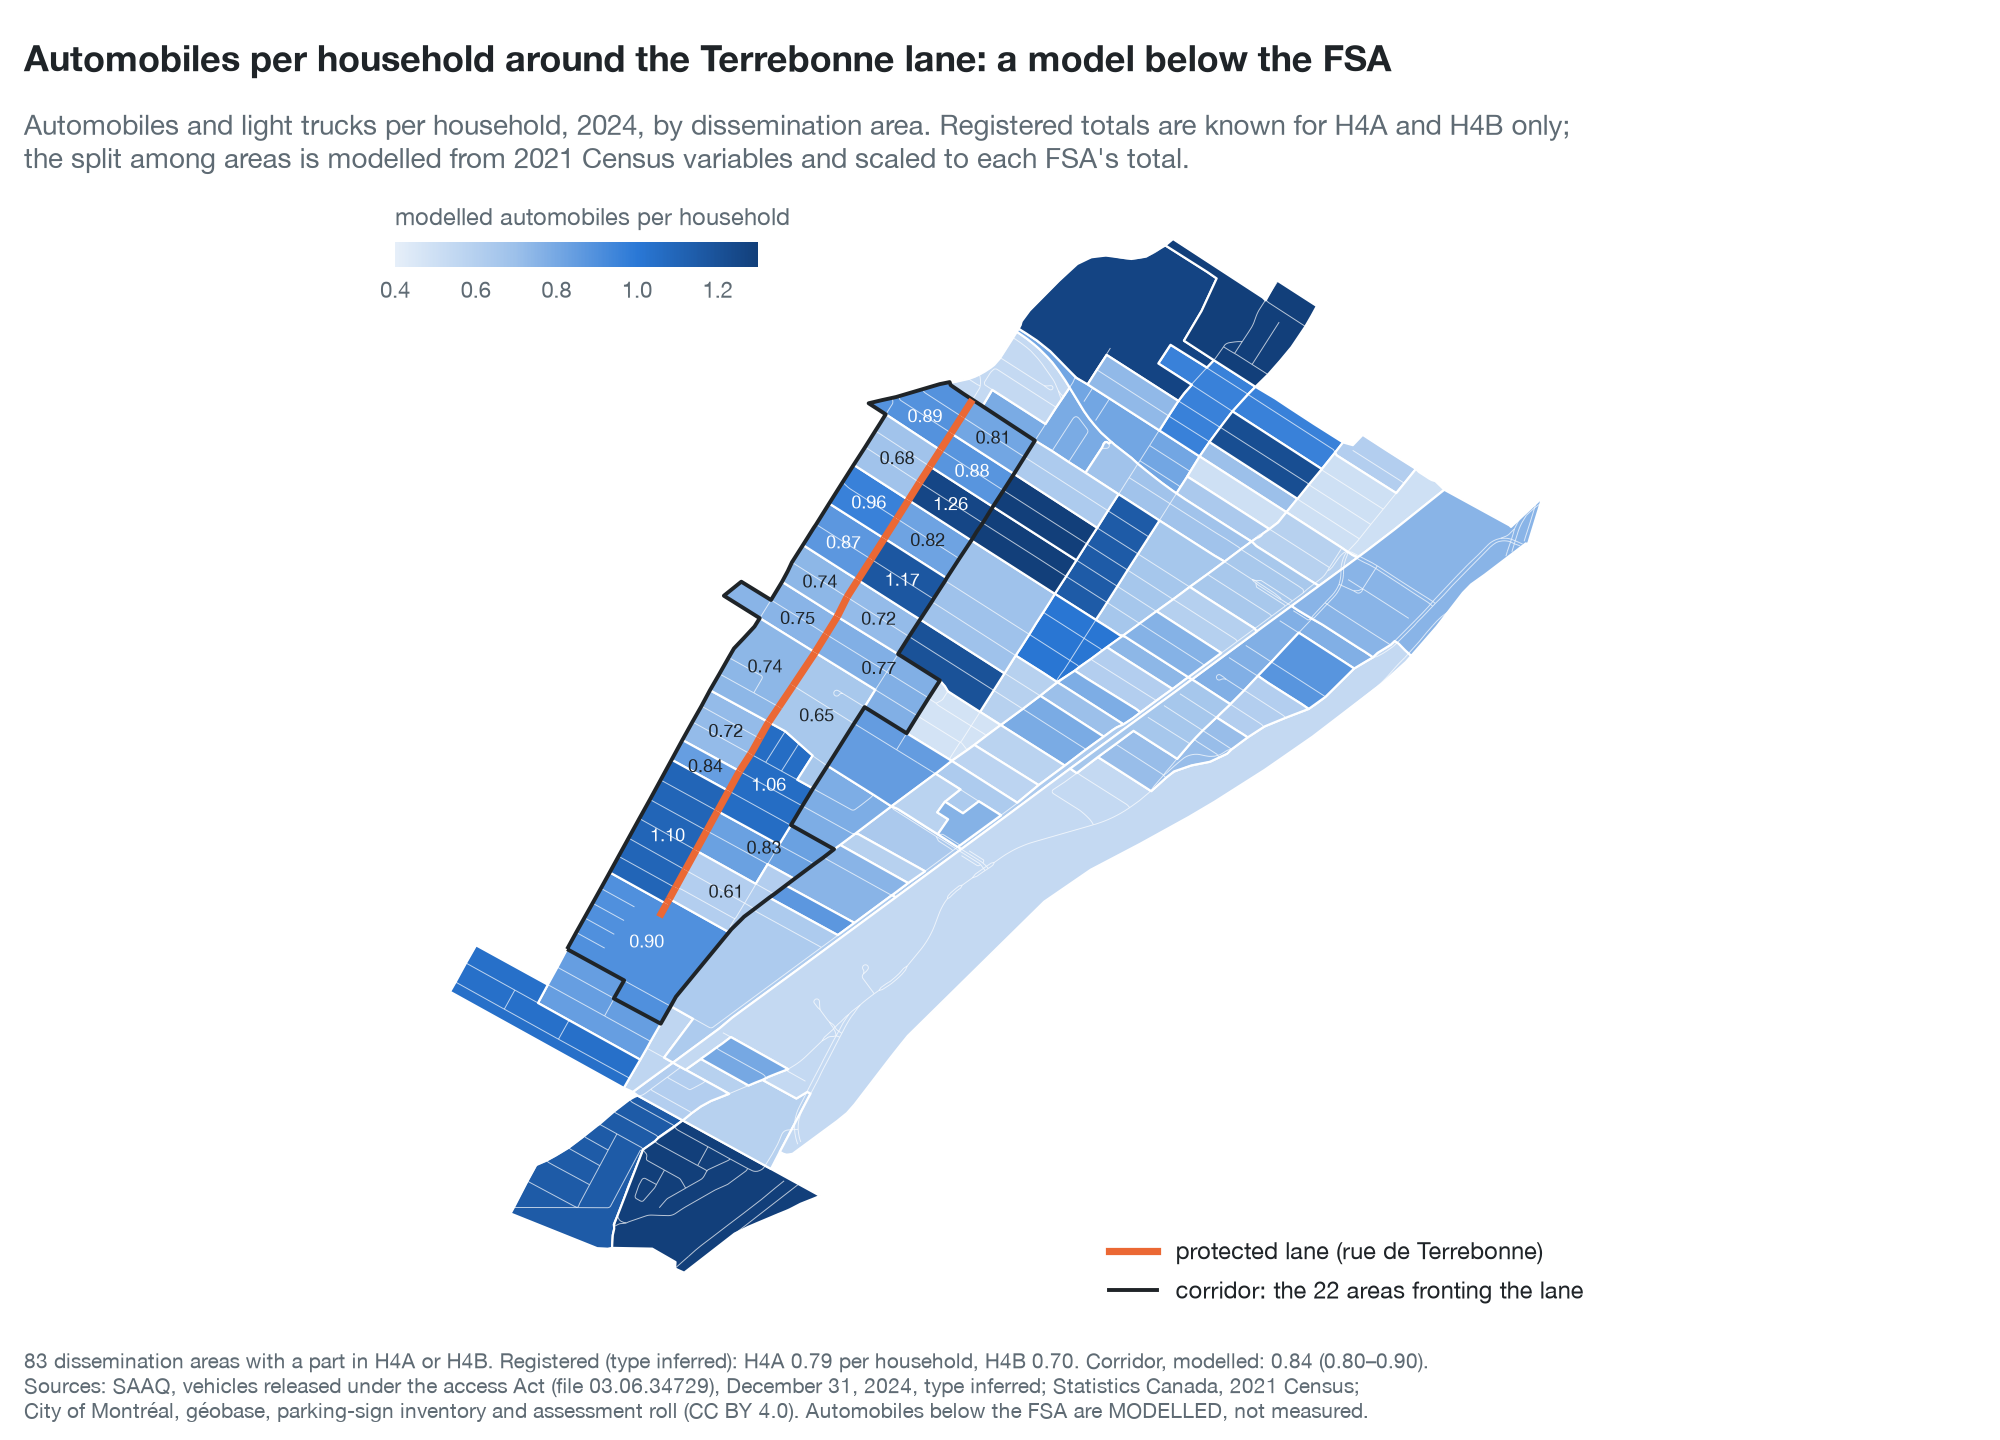
\includegraphics[height=0.74\textheight]{../derived/figures/overview-map/overview_map_en.png}\end{center}
{\footnotesize Registered totals are known for H4A and H4B only. The split among dissemination areas is a model.}
\end{frame}
\begin{frame}{The question}
\begin{itemize}
\item The SAAQ files released under the access Act for 2023 and 2024 locate each vehicle to its \textbf{FSA} (first three characters of the postal code), and no finer.
\item The lane lies in two FSAs: \textbf{H4B} west of Royal (7{,}351 automobiles and light trucks, 0.70 per household) and \textbf{H4A} east of it (9{,}598, 0.79). Type inferred; December 31, 2024.
\item An FSA holds ten to twelve thousand households. What can be said about the areas that front the lane: how many automobiles are registered there, and how much legal curb do they hold?
\item The note makes no recommendation.
\end{itemize}
\end{frame}
\begin{frame}{Two kinds of figures, kept apart}
\begin{columns}[T]
\begin{column}{0.47\textwidth}\textbf{Measured: the curb}
\begin{itemize}\small
\item City géobase and parking-sign inventory (October 2026)
\item Every side of every street segment
\item Less 10\,m at each end (cross street\textquoteright{}s half roadway, and the 5\,m of the Highway Safety Code), less stretches forbidden at all times
\item An \textbf{upper bound}: driveways, hydrants, bus stops, hourly and permit rules not deducted
\end{itemize}\end{column}
\begin{column}{0.47\textwidth}\textbf{Modelled: the automobiles}
\begin{itemize}\small
\item Registered totals exist by FSA only
\item Shared among dissemination areas from 2021 Census variables
\item Scaled so each FSA\textquoteright{}s areas sum to its registered total
\item An \textbf{estimate with an interval}, never a count
\end{itemize}\end{column}\end{columns}
\vspace{1em}The 2015 LiDAR night count and the imagery are a \textbf{check}, not an input.
\end{frame}
\begin{frame}{The corridor}
\begin{itemize}
\item The 22 dissemination areas that hold a block face of rue de Terrebonne along the lane, west end to Girouard.
\item They reach about one block to each side (Somerled about 260\,m north, Monkland about 285\,m south).
\item 5{,}471 households (2021 Census).
\item Dissemination areas do not nest in FSAs: each is shared among FSAs by the dwellings of the City\textquoteright{}s assessment roll in each FSA polygon. Households rebuilt this way: H4A $-$1.2\,\%, H4B $-$1.2\,\% against Statistics Canada\textquoteright{}s own FSA profile.
\end{itemize}
\end{frame}
\begin{frame}{Method: legal curb}
\begin{itemize}
\item A sign governs the stretch from its pole to the next pole in the direction of its arrow; a sign without an arrow, the stretches on both sides.
\item Where the usual reading of the arrows leaves a stretch claimed both by an all-time prohibition and by an hourly rule, the other reading is taken for that face if it leaves fewer such stretches.
\item \textbf{Check on rue de Terrebonne}, where the layout is known: the reading finds one parking band, south side west of Cavendish, north side east of it: 1{,}306\,m, 238 places at 5.5\,m.
\item The borough\textquoteright{}s 2023 study counted 478 places on the two sides before the lane (230 westbound, 248 eastbound).
\end{itemize}
\end{frame}
\begin{frame}{Legal curb by block face}
\begin{center}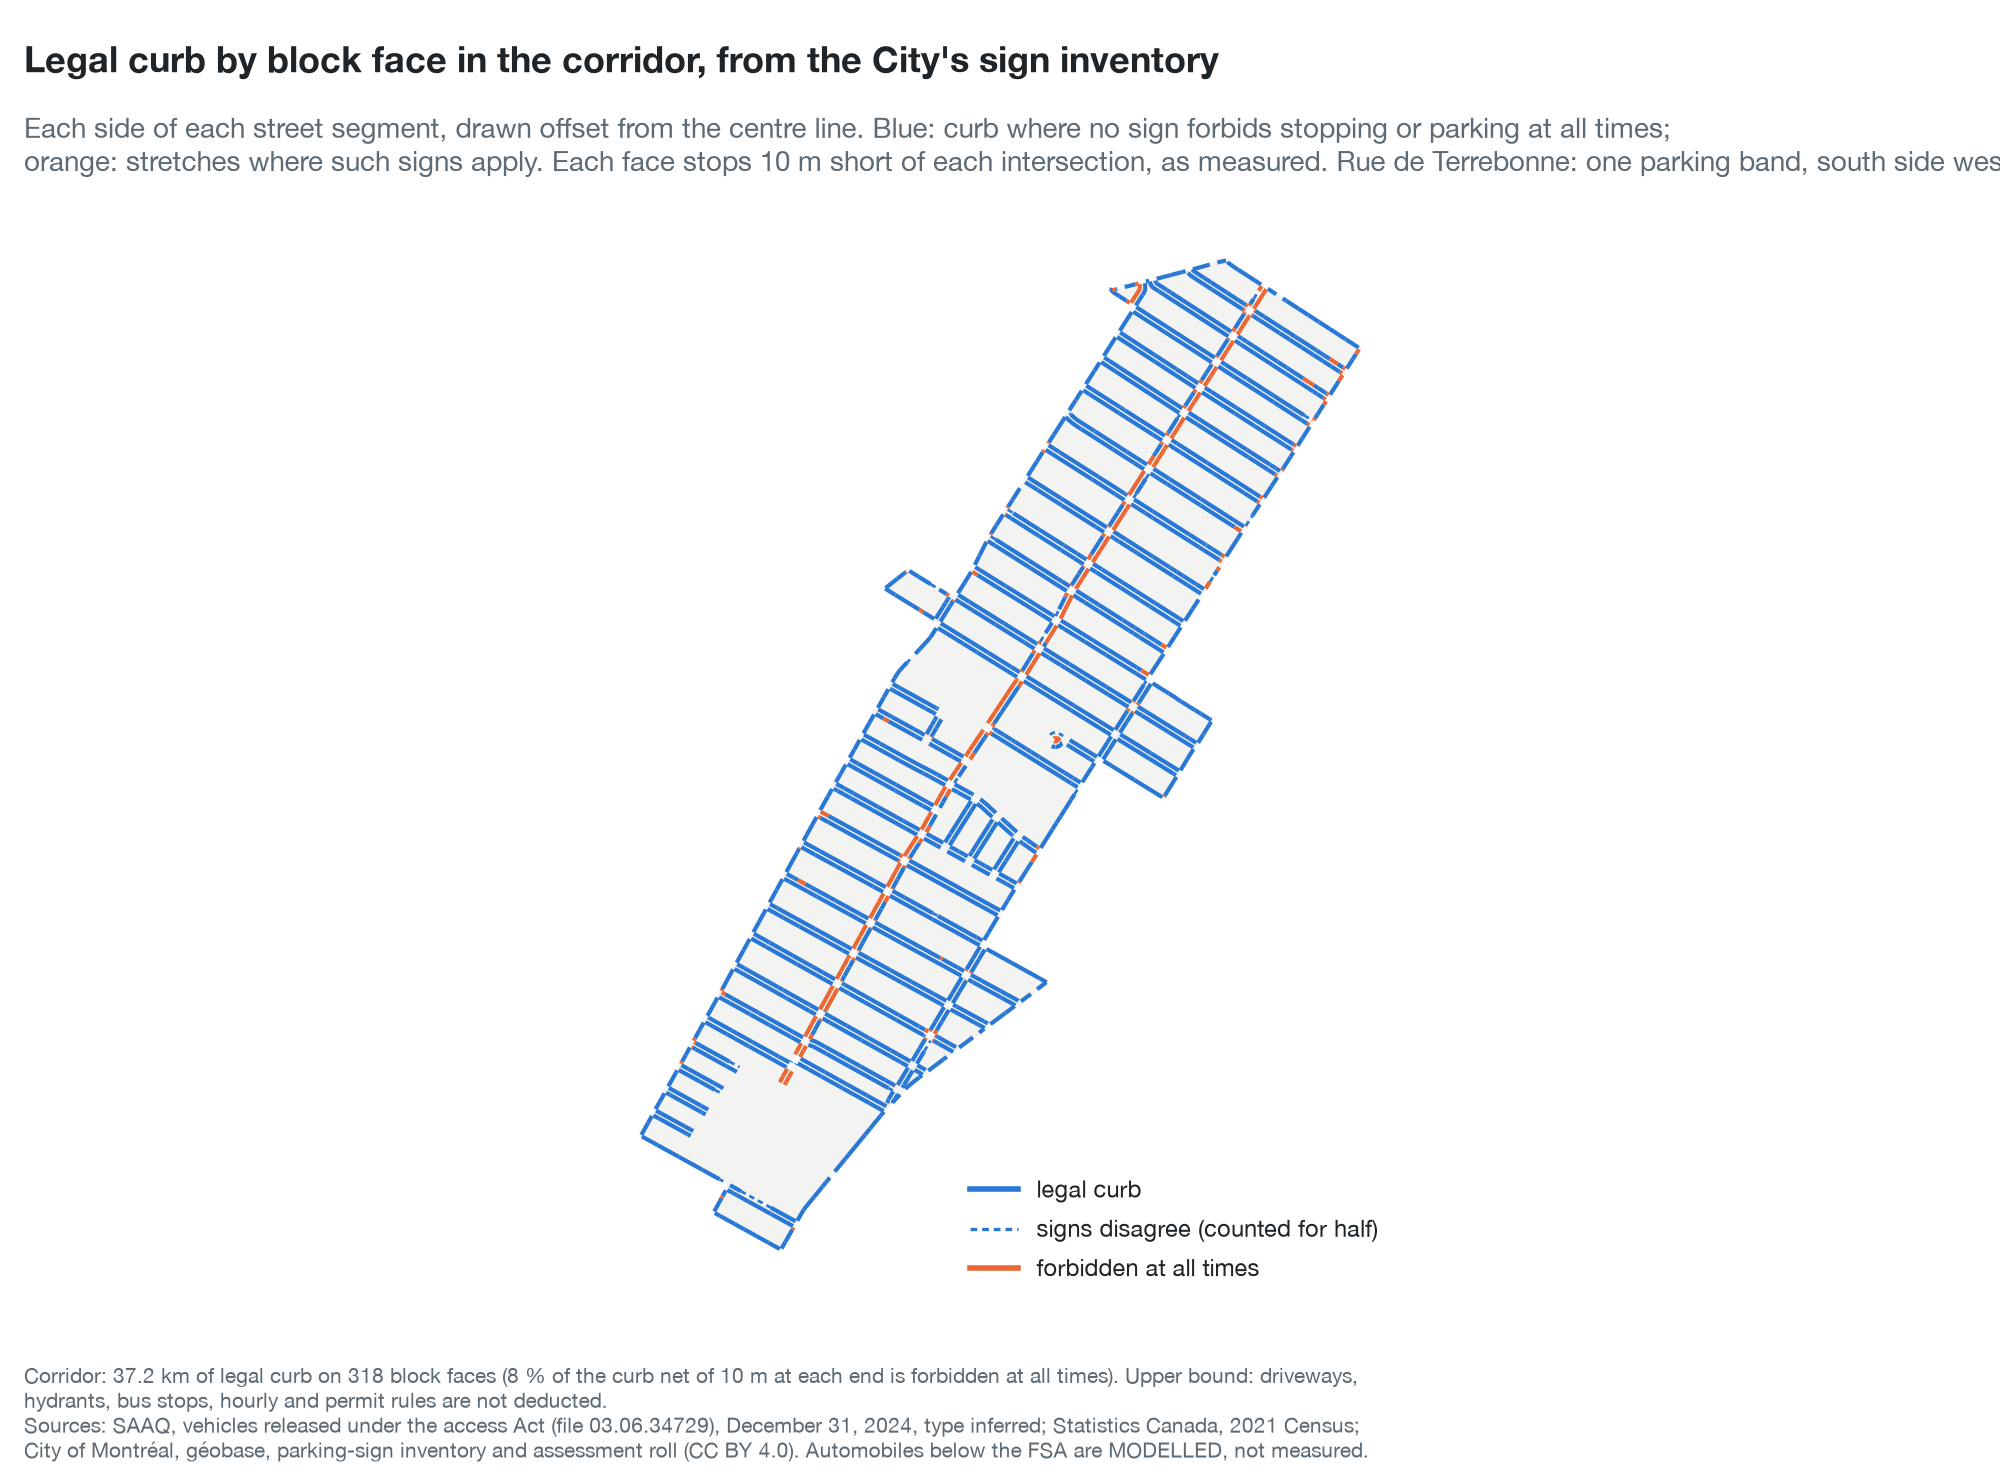
\includegraphics[height=0.7\textheight]{../derived/figures/curb-map/curb_map_en.png}\end{center}
{\footnotesize Corridor: 46.8 km of curb, 37.2 km legal; 6{,}192 to 7{,}431 places at 6 to 5 m (upper bound).}
\end{frame}
\begin{frame}{Method: automobiles below the FSA}
\begin{enumerate}
\item Across 114 FSAs (1{,}000 households or more), the logarithm of automobiles per household is regressed on: share of renters, share of commuters who drive, persons per household, median household income. Robust regression: a few FSAs hold business fleets (H2Y, H2Z, H3A, H3B, H4P, H9P).
\item Each dissemination area\textquoteright{}s rate is predicted from its own census variables.
\item Predictions are scaled so each FSA\textquoteright{}s areas sum to its registered total (factors 1.07 for H4A, 0.99 for H4B).
\end{enumerate}
\textbf{Intervals}: 2{,}000 draws (FSAs resampled; sampling error of the 25\,\% sample variables; an unexplained factor per area; rescaling).

Not covered by the intervals: census of 2021 against vehicles of 2024; inferred type; vehicles registered to businesses.
\end{frame}
\begin{frame}{Does the model work where the answer is known?}
\begin{center}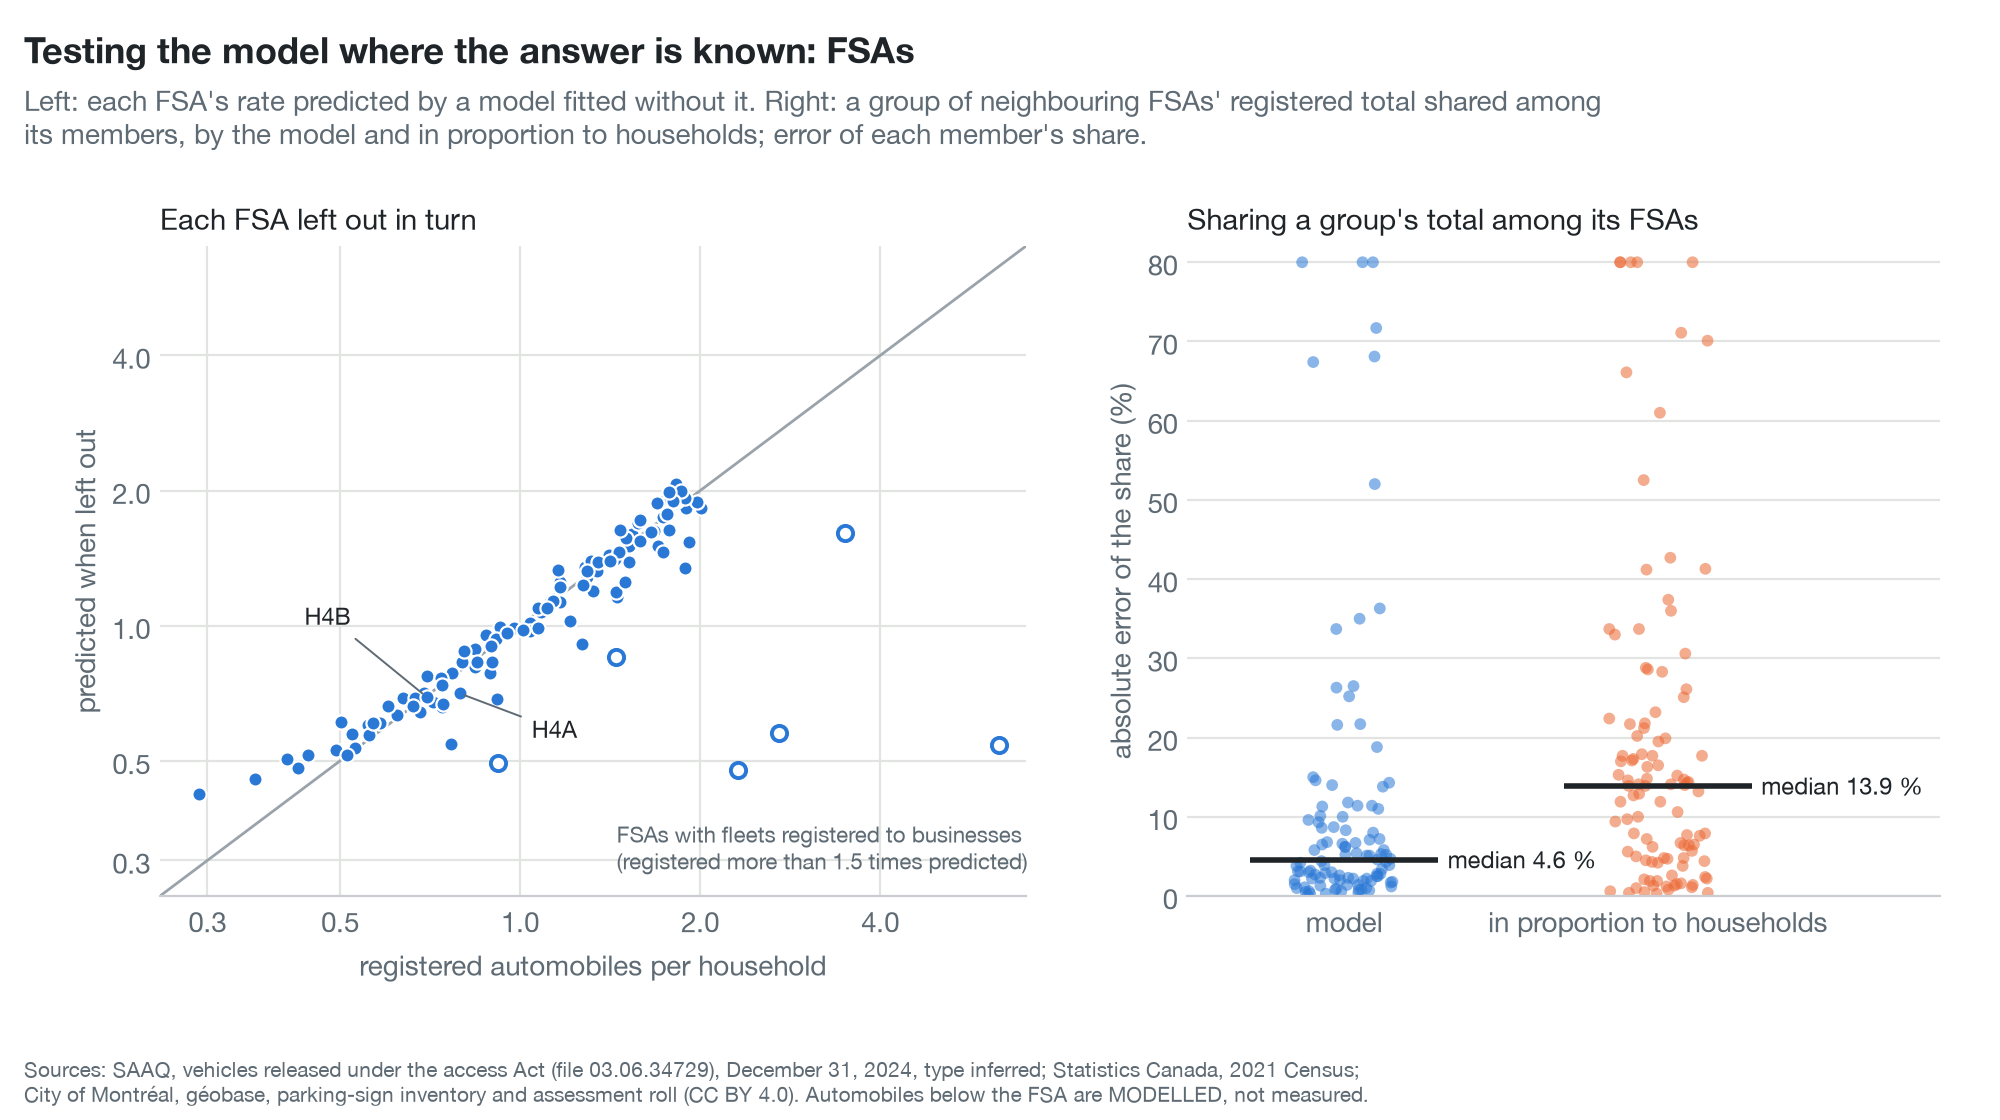
\includegraphics[height=0.6\textheight]{../derived/figures/model-tests/model_tests_en.png}\end{center}
{\footnotesize Sharing a group of FSAs\textquoteright{} total among its members: off by 4.6\,\% at the median with the model, 13.9\,\% in proportion to households. For H4A and H4B as a pair the model gains little. Below the FSA nothing can test the split.}
\end{frame}
\begin{frame}{The corridor: modelled automobiles, measured curb}
\begin{center}\resizebox{0.98\textwidth}{!}{\begin{tabular}{lrrrrrrrr}\toprule
 & areas & households & automobiles & 90\,\% interval & per household & legal curb km & places (6 to 5\,m) & per place (5.5\,m) \\\midrule
Corridor & 22 & 5{,}471 & 4{,}622 & 4{,}382--4{,}927 & 0.84 & 37.2 & 6{,}192--7{,}431 & 0.68 \\
Other areas of H4A, H4B & 61 & 18{,}978 & 14{,}363 & 14{,}033--14{,}641 & 0.76 & 109.3 & 18{,}210--21{,}852 & 0.72 \\
All & 83 & 24{,}449 & 18{,}985 & 18{,}830--19{,}163 & 0.78 & 146.4 & 24{,}402--29{,}283 & 0.71 \\
\bottomrule\end{tabular}}\end{center}
\begin{itemize}
\item Corridor: 0.84 automobile per household (0.80 to 0.90); the other areas of the two FSAs, 0.76.
\item The two alternative specifications give 4{,}616 and 4{,}683 for the corridor.
\item Places are an upper bound; automobiles are every vehicle registered, wherever it is kept.
\end{itemize}
\end{frame}
\begin{frame}{Area by area: the estimates and their intervals}
\begin{center}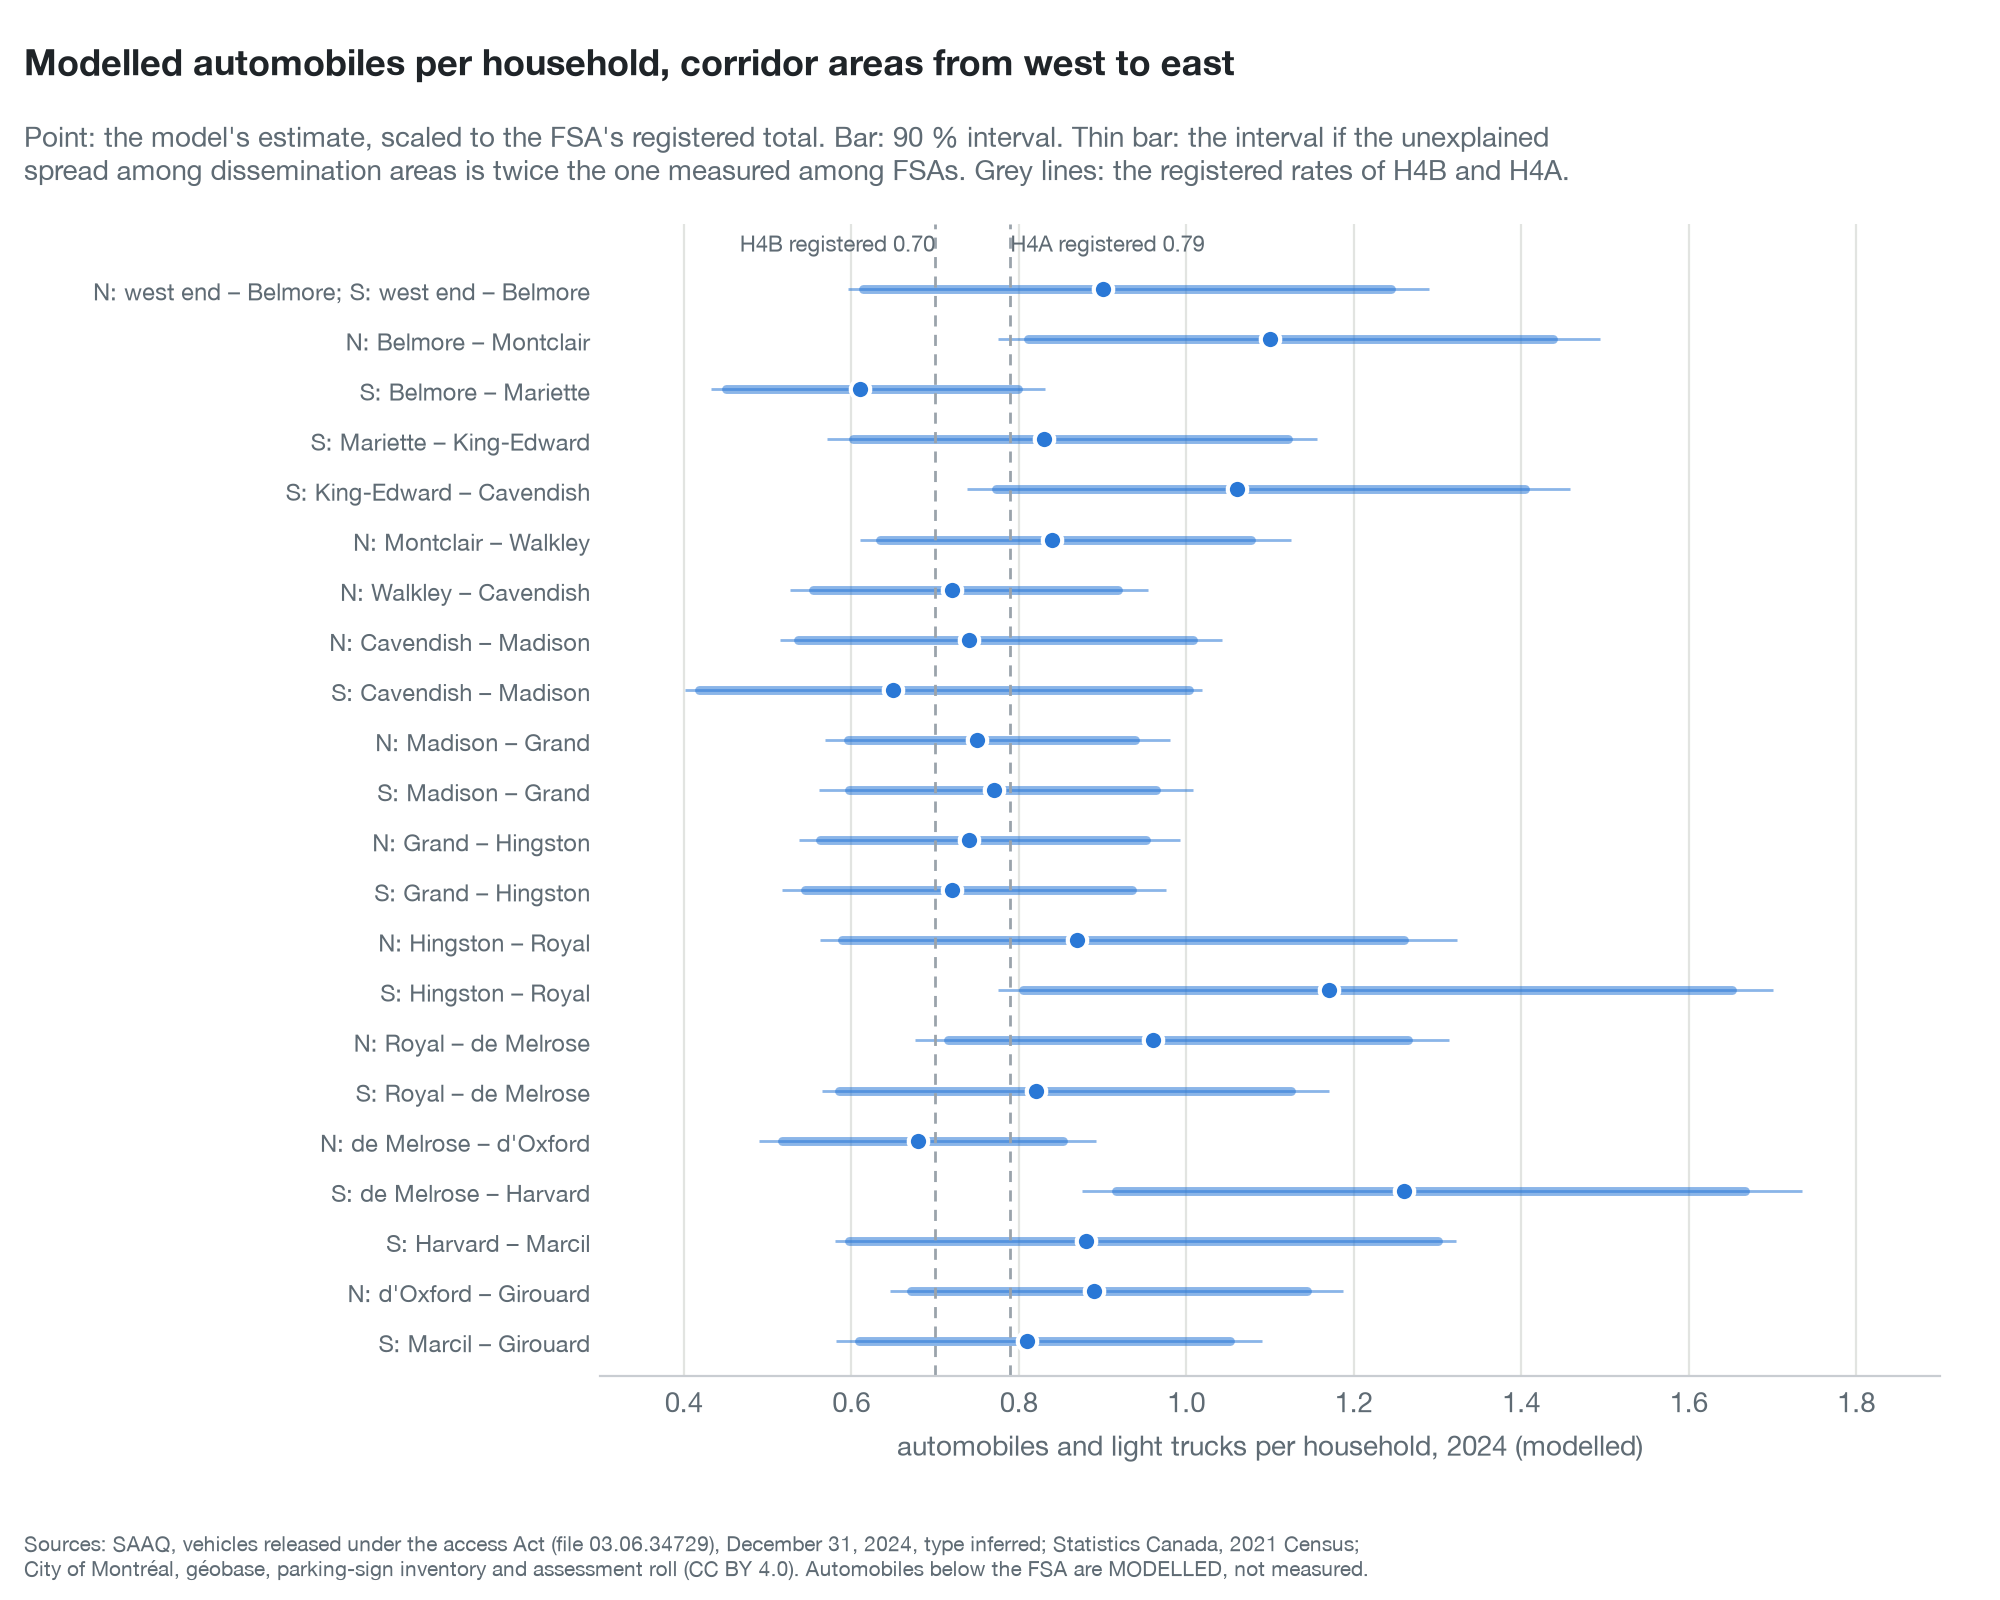
\includegraphics[height=0.7\textheight]{../derived/figures/area-estimates/area_estimates_en.png}\end{center}
{\footnotesize A single area\textquoteright{}s 90\,\% interval is about 29\,\% of its estimate either way; most differences between neighbours are within it.}
\end{frame}
\begin{frame}{Modelled automobiles beside the places the legal curb would hold}
\begin{center}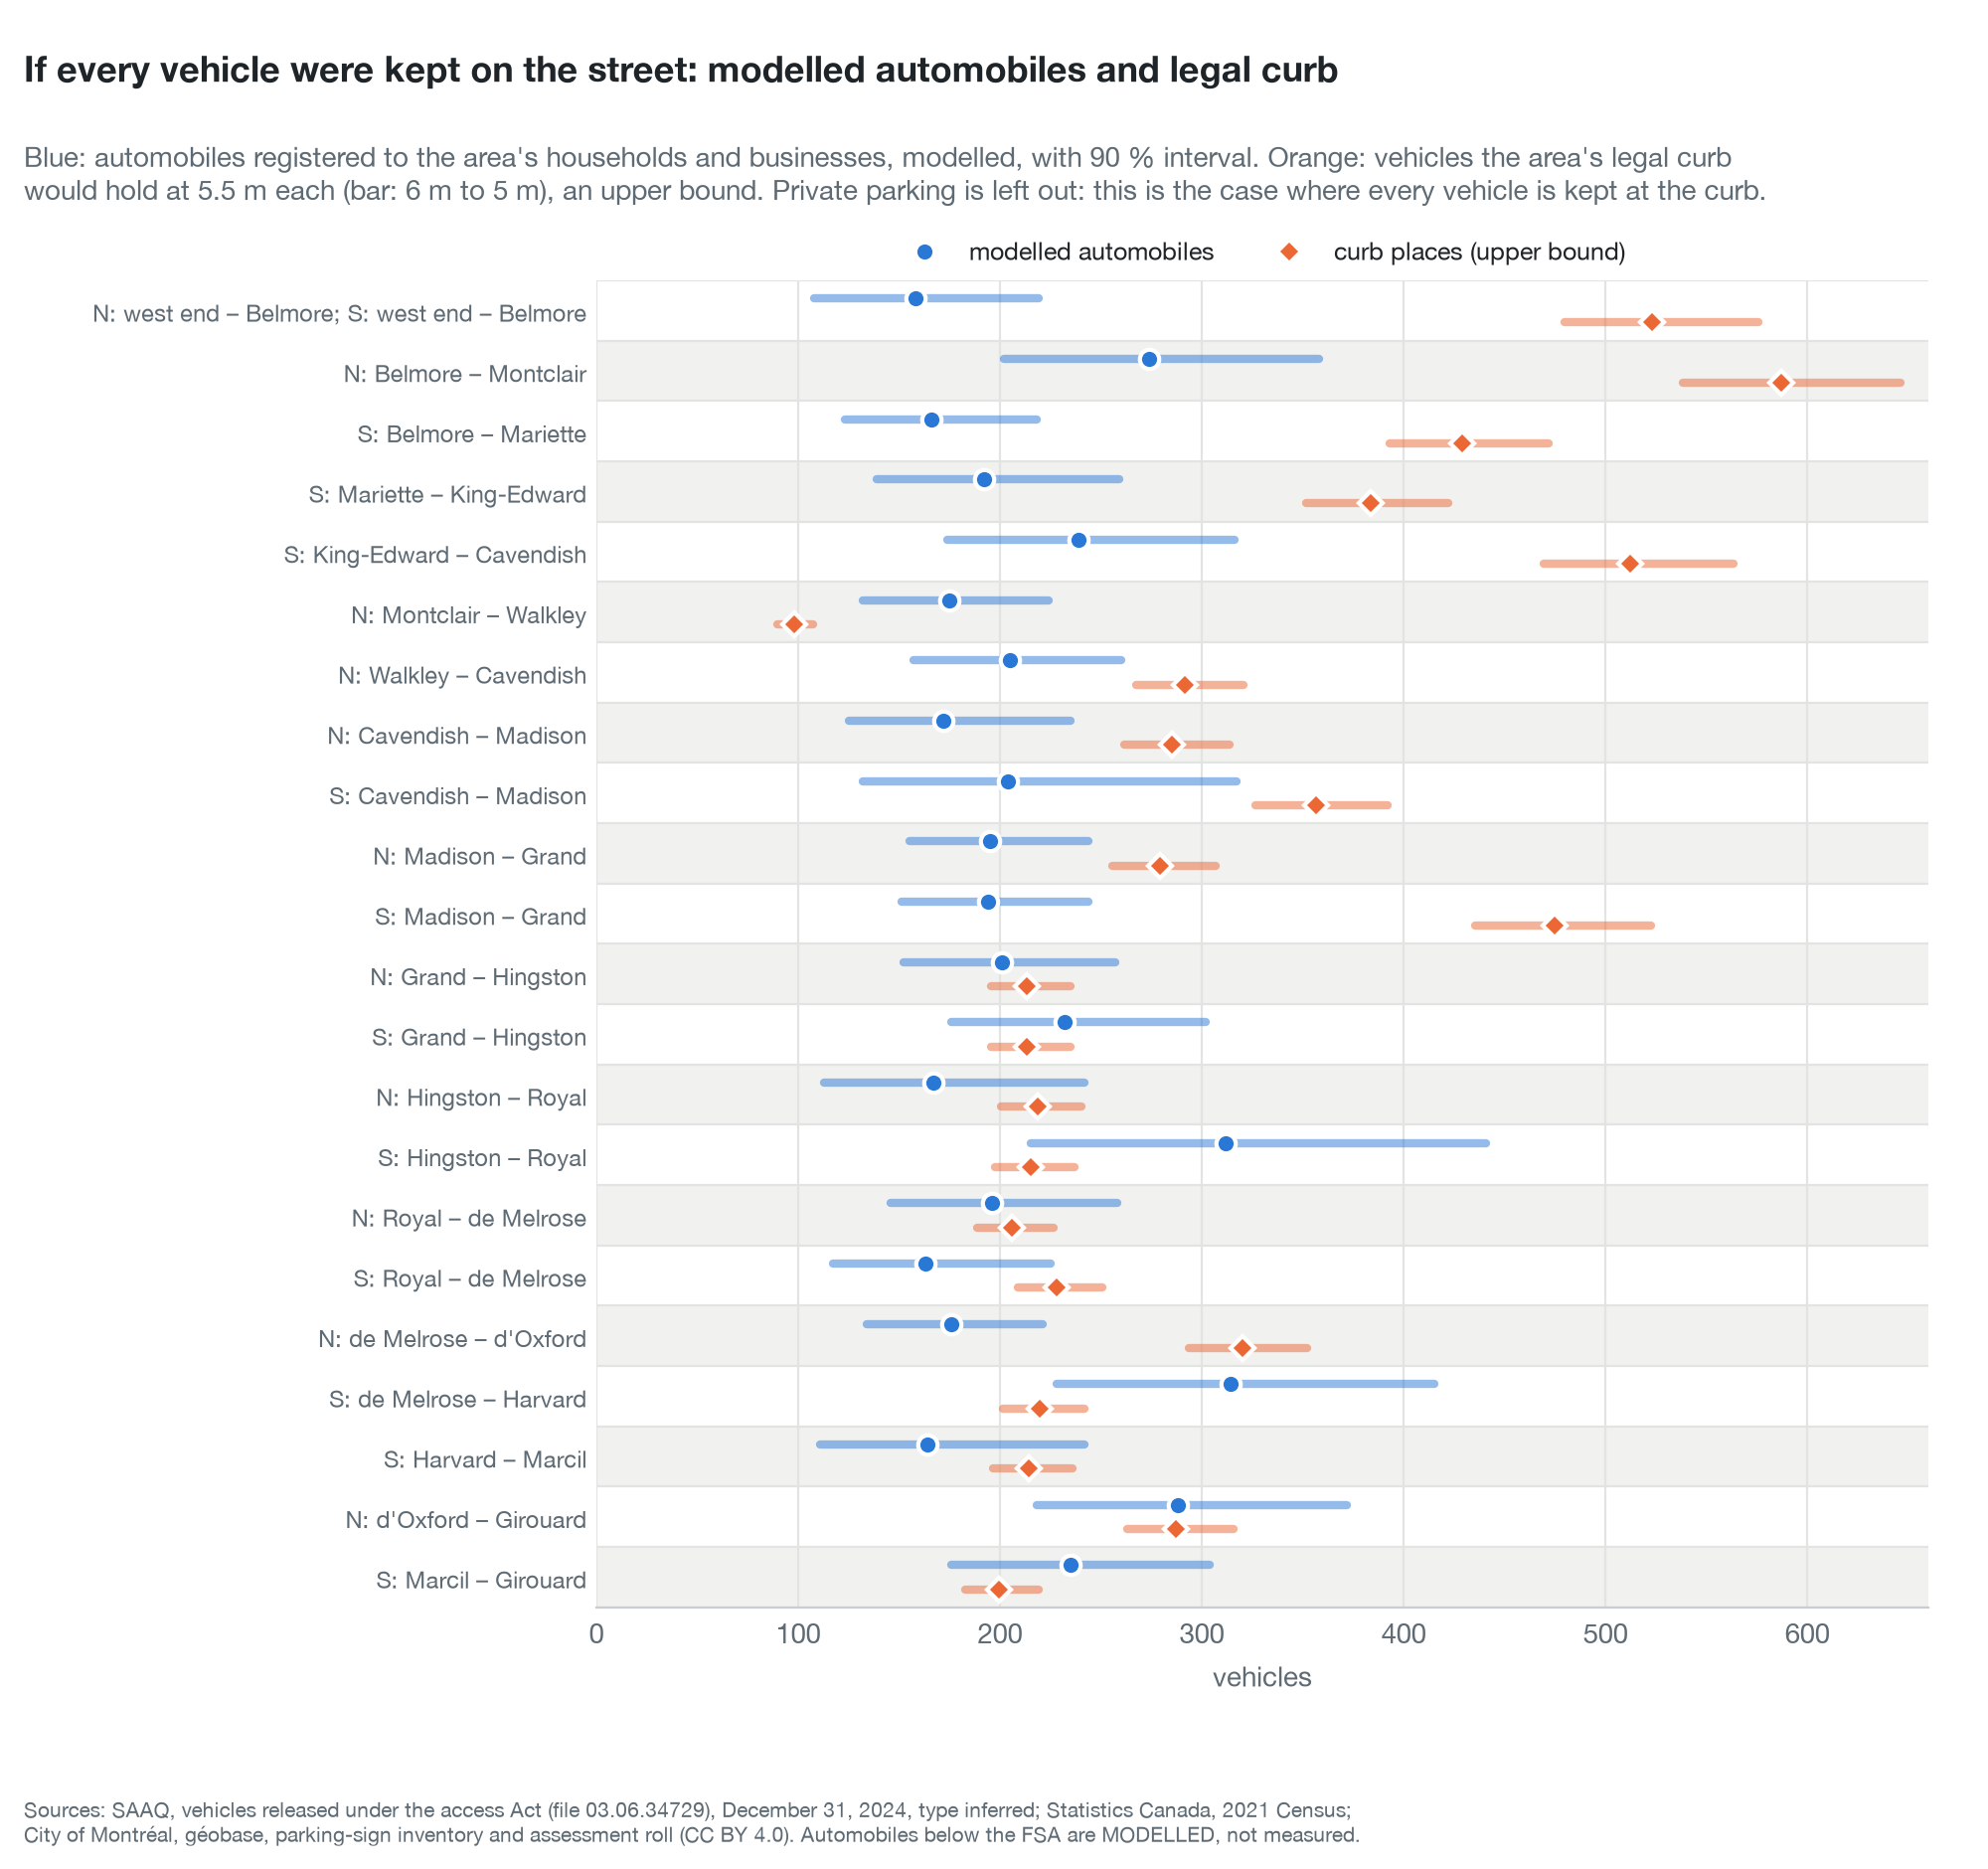
\includegraphics[height=0.76\textheight]{../derived/figures/curb-and-automobiles/curb_and_automobiles_en.png}\end{center}
\end{frame}
\begin{frame}{Why the ratio is not a measure of parking pressure}
\begin{itemize}
\item At 5.5\,m per place: 0.68 modelled automobile per place of legal curb in the corridor (0.65 to 0.73); the estimate exceeds the area\textquoteright{}s own places in 6 of 22 areas.
\item The curb figure is an \textbf{upper bound}: no driveway, hydrant, bus stop, hourly or permit rule deducted.
\item This comparison is the limiting case where \textbf{every registered vehicle is kept at the curb}. Private parking: next slides.
\item Visitors, institutions and vehicles from elsewhere use the same curb; a place at the far end of an area is not a place at one\textquoteright{}s door.
\item The occupancy measurements that exist are EXP\textquoteright{}s: Thursday, September 29, 2022, 18:30--19:30: 247 cars on Terrebonne\textquoteright{}s places (50\,\%), 311 on the cross-street stubs (51\,\%).
\end{itemize}
\end{frame}
\begin{frame}{Private parking, measured on rue de Terrebonne}
\begin{center}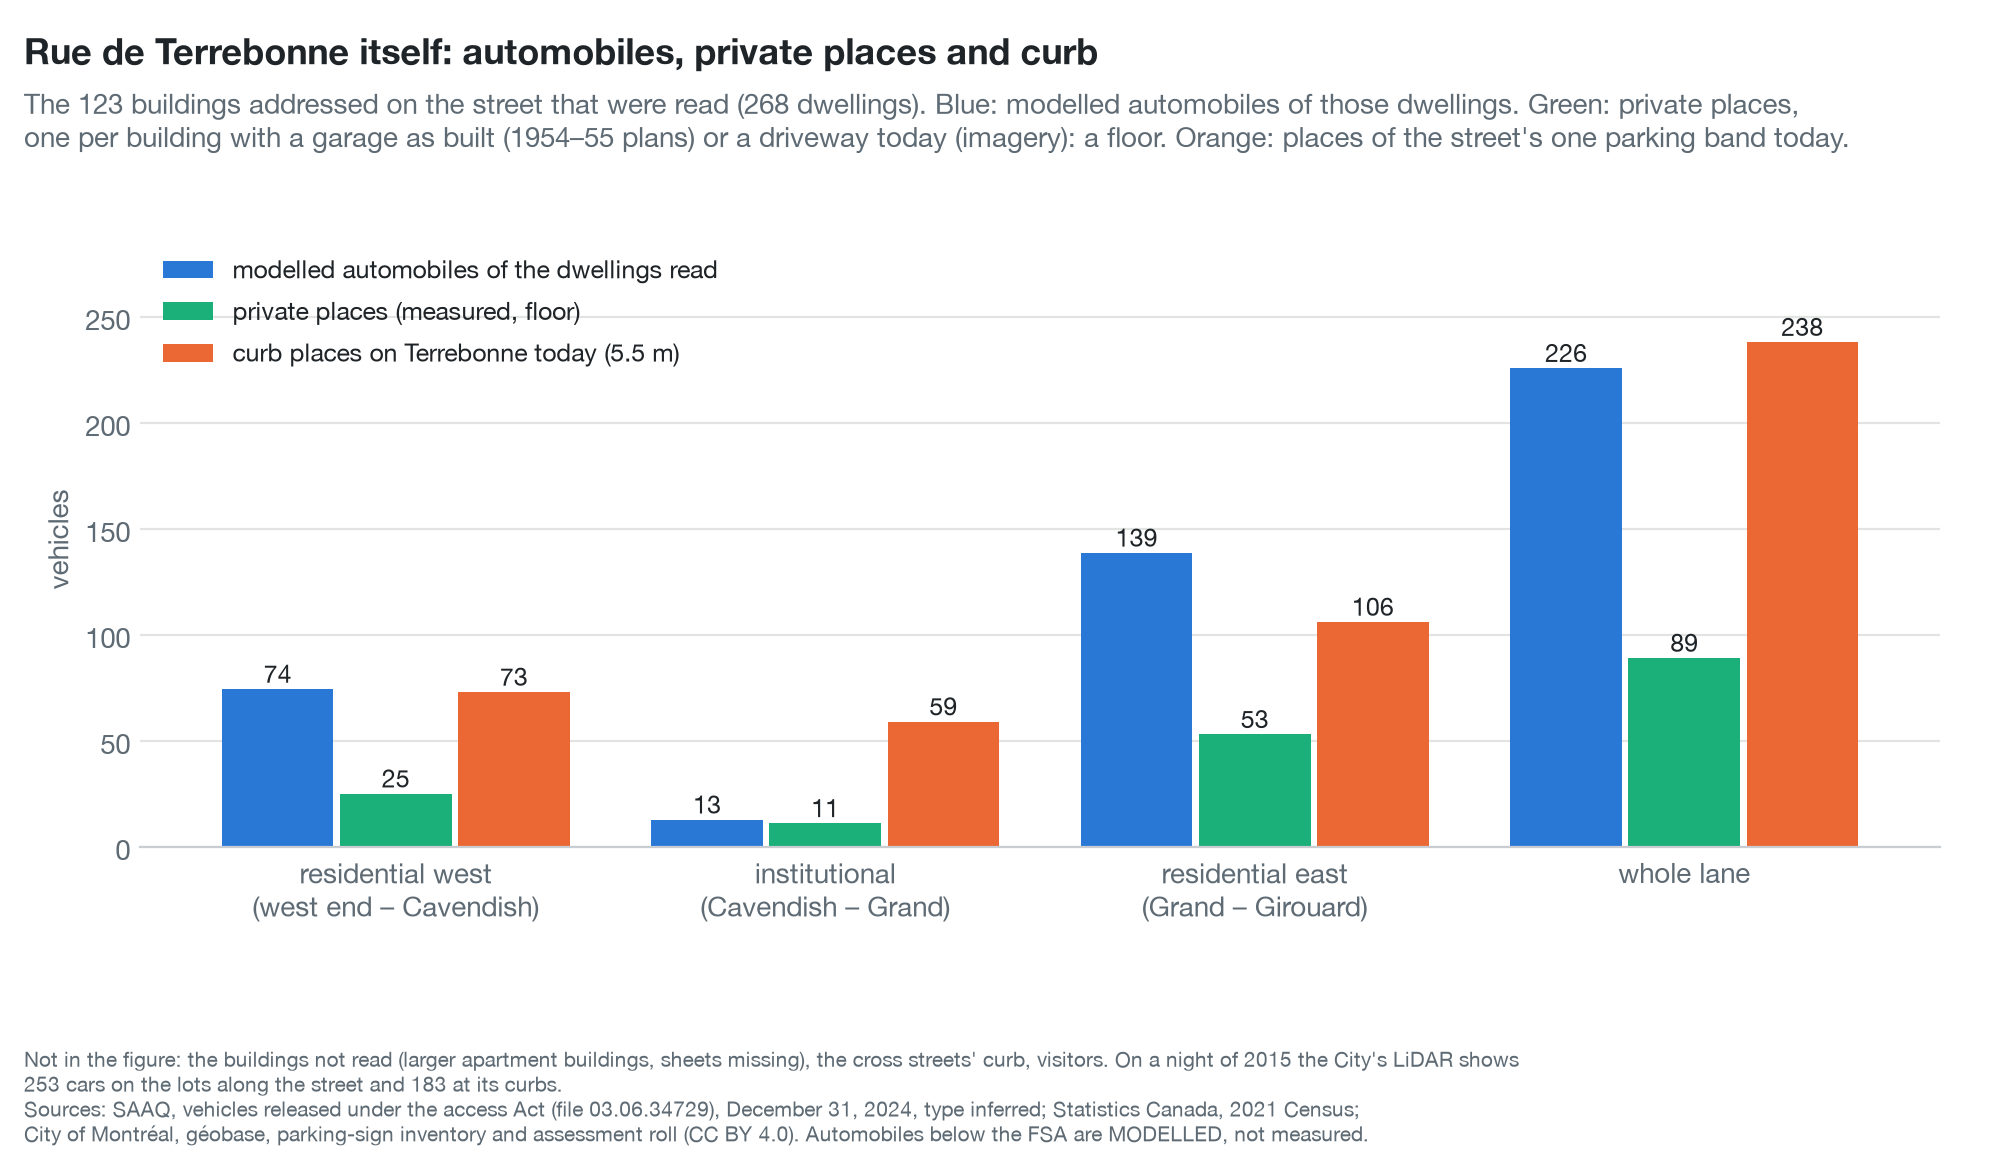
\includegraphics[height=0.6\textheight]{../derived/figures/off-street-terrebonne/off_street_terrebonne_en.png}\end{center}
{\footnotesize 89 of the 123 buildings read have a garage as built or a driveway today (72\,\%). One place is counted per such building.}
\end{frame}
\begin{frame}{Private parking in the corridor: every lot read, then checked}
\begin{itemize}
\item Every lot holding a dwelling (2{,}358) was read on enlarged aerial crops by independent readers under a written protocol. A first reading failed its checks and was redone.
\item A random sample of 112 lots, drawn beforehand, was judged by the author from street-level imagery without seeing the readers\textquoteright{} answers.
\item Small buildings in the check: \textbf{85 of 99 have car access} (86\,\%). Where the readers said yes, the check confirmed 52 of 56; where they said no, only 8 of 23: a view from above misses driveways.
\item Estimate for the 2{,}262 small buildings, calibrated on the check: \textbf{2{,}228 private places} a car can leave without another being moved (2{,}051 to 2{,}414); 3{,}731 with cars one behind another. Garage interiors not counted.
\item The 96 buildings of six dwellings or more are given none: 6 of the 12 checked have an underground garage that cannot be counted.
\end{itemize}
\end{frame}
\begin{frame}{With private parking added, area by area}
\begin{center}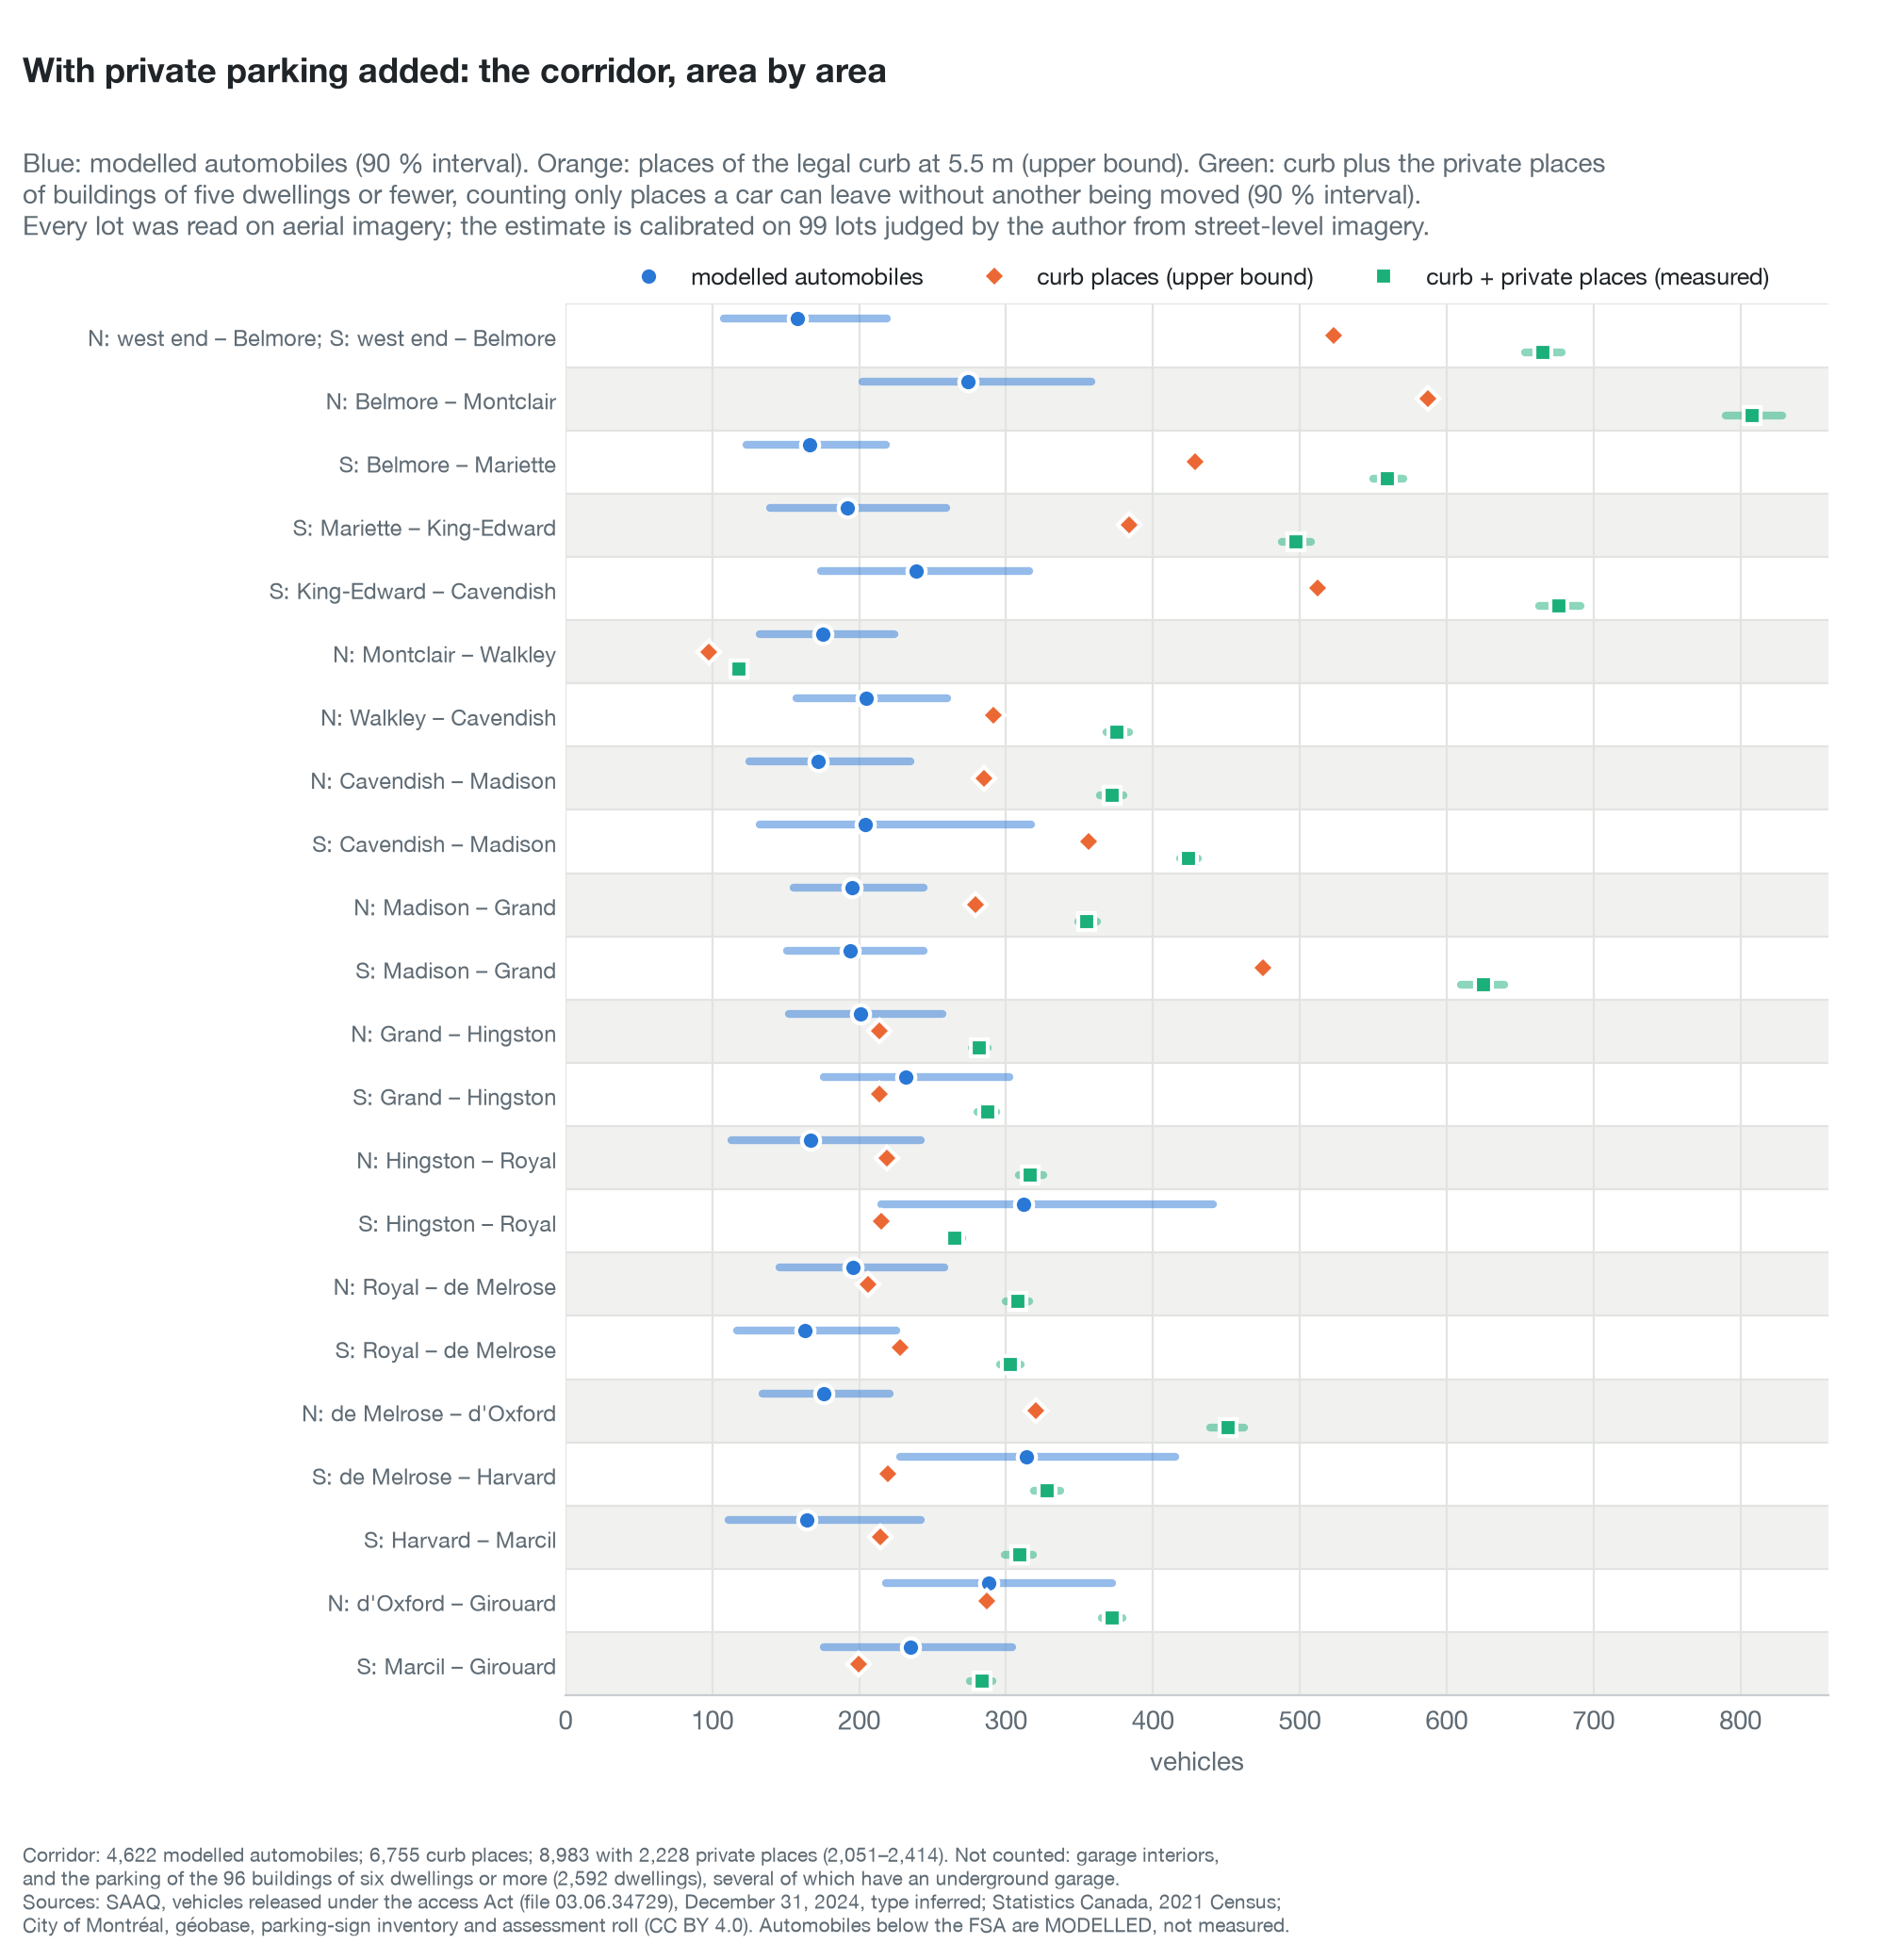
\includegraphics[height=0.7\textheight]{../derived/figures/off-street-corridor/off_street_corridor_en.png}\end{center}
{\footnotesize 0.51 modelled automobile per place with private places, against 0.68 with the curb alone.}
\end{frame}
\begin{frame}{A check from another source: the 2015 LiDAR night}
\begin{center}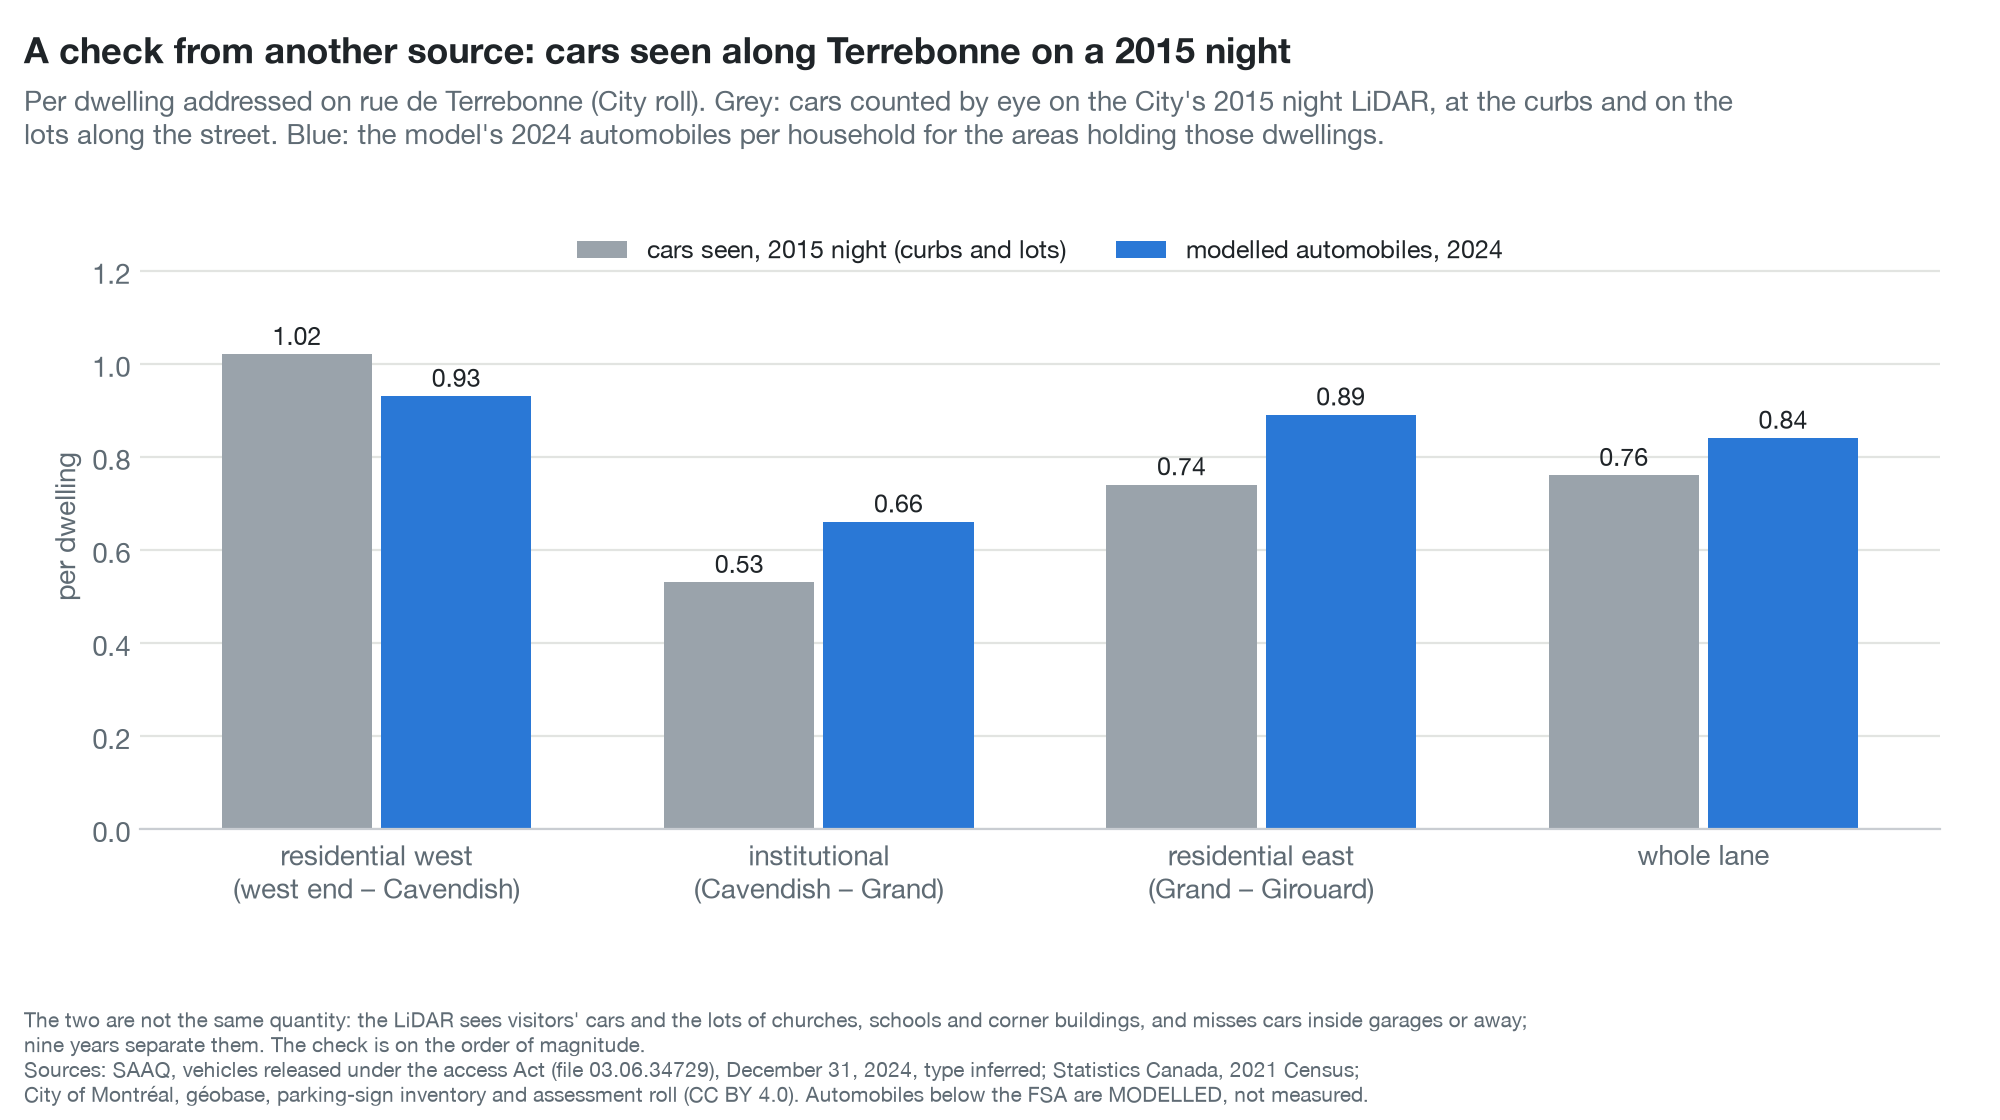
\includegraphics[height=0.6\textheight]{../derived/figures/lidar-check/lidar_check_en.png}\end{center}
{\footnotesize 436 cars seen for 573 dwellings addressed on Terrebonne. Agreement in order of magnitude; area by area, no relation (rank correlation 0.31, 11 areas).}
\end{frame}
\begin{frame}{What is shown and what is not}
\begin{itemize}
\item \textbf{Measured:} the registered automobiles of H4A and H4B (type inferred); the legal curb of each block face, as an upper bound; garages and driveways on rue de Terrebonne.
\item \textbf{Measured, with a measured error:} private places of small buildings (every lot read, a random sample checked from the street).
\item \textbf{Not counted:} garage interiors; the garages of larger buildings.
\item \textbf{Modelled:} the automobiles of every area smaller than an FSA. The model shares a known total better than households alone where that can be tested; below the FSA nothing can test it, and the 2015 check does not confirm its area-by-area differences.
\item \textbf{Not measured by anyone:} where registered vehicles are kept; occupancy of the curb since the lane was built.
\end{itemize}
\end{frame}
\begin{frame}{Where everything is}
\begin{itemize}
\item Note, tables by dissemination area and by block face, figures (English and French) and scripts: \url{https://github.com/OpenMobilityData/Terrebonne-open-sources/tree/main/2026-terrebonne-corridor-vehicles-and-curb}
\item Sources: SAAQ (access request 03.06.34729; tables of Quebec-vehicle-registrations); Statistics Canada, 2021 Census; City of Montréal open data (géobase, parking-sign inventory, assessment roll, LiDAR 2015; CC BY 4.0); DMTI Spatial (FSA polygons, under licence).
\end{itemize}
\end{frame}

\end{document}
